
\section{Motivation and Scope}

\subsection{Usefullness of reflection}

There is a wide range of computer programming tasks that involve
the execution of the same algorithm on a set of types defined by an
application or on instances of these types, accessing member variables,
calling free or member functions in an uniform
manner, converting data between the language's intrinsic representation and
external formats, etc., for the purpose of implementing the following:

\begin{itemize}

\item serialization or storing of persistent data in a
custom binary format or in XML, JSON, XDR, etc.,

\item (re-)construction of class instances
from external data representations (like those listed above),
from the data stored in a relational database, from data entered by
a user through a user interface or queried through a web service API,

\item automatic generation of a relational schema from the application
object model and object-relational mapping (ORM),

\item support for scripting 

\item support remote procedure calls (RPC) / remote method invocation (RMI),

\item inspection and manipulation of existing objects via a (graphic) user interface
or a web service,

\item visualization of objects or data and the relations between objects or
relations in the data,

\item automatic or semi-automatic implementation of certain software design patterns,

\item etc.

\end{itemize}

There are several aproaches to the implementation of such
functionality. The most straightforward and also usually the most
error-prone is manual implementation. Many of the tasks listed above
are inherently repetitive and basically require to process programming
language constructs (types, structures, containers, functions, constructors,
class member variables, enumerated values, etc.)
in a very uniform way that could be easily transformed into a meta-algorithm.

While it is acceptable (even if not very advantageous)
for example, for a design pattern implementation to be made by a human,
writing RPC/RMI-related code is a task much better suited for a computer.

This leads to the second, heavily used approach: preprocessing
and parsing of the program source text by a (usually very specfic) external
program (documentation generation tool, interface definition language compiler
for RPC/RMI, web service interface generator, a rapid application
development environment with a form designer, etc.) resulting in additional
program source code, which is then compiled into the final application binary.

This approach has several problems. First, it requires the external
tools which may not fit well into the build system or may not be portable
between platforms or be free; second, such tools are task-specific
and many of them allow only a limited, if any, customization of the output.

Another way to automate these tasks is to use reflection,
reflective programming, metaprogramming and generic programming as
explained below.

\subsection{Motivational examples}

This section describes some of the many possible uses of reflection
and reflective programming on concrete real-world examples.

\subsubsection{Factory generator}

As already said above, it is possible (at least partially) to automate 
the implementation of several established software design patterns.
This example shows how to implement a variant of the {\em Factory}
pattern.

By factory we mean here a class, which can create
instances of a {\em Product} type, but does not require that
the caller chooses the manner of the construction (in the programming
language) nor supplies the required arguments directly
in the C++ intrinsic data representation.

So instead of direct construction of a Product type,

\begin{lstlisting}
// get the values of arguments from the user
int arg1 = get_from_user<int>("Product arg1");
double arg2 = get_from_user<double>("Product arg2");
std::string arg3 = get_from_user<std::string>("Product arg3");
//
// call a constructor with these arguments
Product* pp = new Product(arg1, arg2, arg3);
// default construct a Product
Product p;
// copy construct a Product
Product cp = p;
\end{lstlisting}

which involves selection of a specific constructor, getting
the values of the required arguments and possibly converting 
them from an external representation and calling the selected
constructor with the arguments, 
factories pick or let the application user pick the Product's most
appropriate constructor, they gather the necessary parameters
in a generic way and use the selected constructor to create
an instance of the Product:

\begin{lstlisting}
// get data necessary for construction in xml
XMLNode xml_node_1 = get_xml_node(...);
XMLNode xml_node_2 = get_xml_node(...);

// make a factory for the product type
Factory<Product, XMLWalker> xml_factory;

// use the factory to create instances of Product
// from the external representation
Product p = xml_factory(xml_node_1);
Product* pp = xml_factory.new_(xml_node_2);
\end{lstlisting}

One of the interesting features of these factories is,
that they separate the caller (who just needs to get an instance
of the specified type) from the actual method of creation.

By using a factory, the constructor to be called can 
be automatically picked depending on the data available only at run-time
and not be chosen by the programmer (at least not directly
as in the code above). Factory can match
the constructor to best fit the data available in the external
representation (XML or JSON fragment, dataset resulting from a
RDBS query, etc.)

Even more interesting is, that such factories can be
implemented semi-automatically with the help of reflection.

Every factory is a composition of two distinct (and nearly orthogonal)
parts:

\begin{itemize}
\item{Product-type-dependent}: includes the enumeration of Product's
constructors, enumeration of their parameters, information about
the context in which a constructor is called, etc. This part is based
on reflection and independent on the representation of the input data.

\item{Data representation-dependent}: includes the scanning of the
available input data, conversion into C++ intrinsic data representation,
and the selection of the best constructor. This part is user-defined
and specifies how the input data is gathered and converted into the
C++ representation.
\end{itemize}

\begin{figure}[!th]
\centering
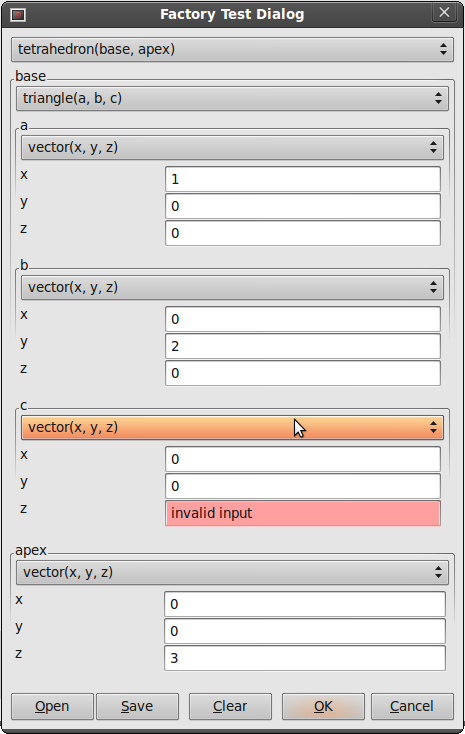
\includegraphics[width=.5\textwidth]{fact_tetrahedron.png}
\caption{Example of a GUI created by a factory generated by
the Mirror's factory generator.}
\label{fig:fact-tetrahedron}
\end{figure}

These two parts are then tied together into the factory class. Based
on the input-data related components, the factory can include a script parser
or XML document tree walker or code dynamically generating a GUI
for the input of the necessary values and the selection of the preferred
constructor. Figure \ref{fig:fact-tetrahedron} shows such a GUI created
by factory automatically generated by the Mirror's {\em factory generator}
utility for a tetrahedron class with the following definition:

\begin{lstlisting}
struct vector
{
        double x,y,z;

        vector(double _x, double _y, double _z)
         : x(_x), y(_y), z(_z)
        { }

        vector(double _w)
         : x(_w), y(_w), z(_w)
        { }

        vector(void)
         : x(0.0), y(0.0), z(0.0)
        { }

        /* other members */
};

struct triangle
{
        vector a, b, c;

        triangle(
		const vector& _a,
		const vector& _b,
		const vector& _c
	): a(_a), b(_b), c(_c)
        { }

        triangle(void){ }

        /* other members */
};

struct tetrahedron
{
        triangle base;
        vector apex;

        tetrahedron(const triangle& _base, const vector& _apex)
         : base(_base), apex(_apex)
        { }

        tetrahedron(
                const vector& a,
                const vector& b,
                const vector& c,
                const vector& d
        ): base(a, b, c), apex(d)
        { }

        /* other members */
};

\end{lstlisting}

